\documentclass{ufersa}

\begin{document}

\section{Introdução}

O presente relatório está organizado da seguinte maneira: primeiramente, são explicados os ambientes tecnológicos que são estudados e trabalhados e depois o relatório divide-se em duas partes. Na Parte 1 está relatado o desenvolvimento do aplicativo Bee comerciais, aplicativo ao qual o estagiário foi desenvolvedor, atualmente o aplicativo já está concluído e sendo utilizado, sendo possível baixá-lo diretamente das lojas virtuais Google Store e Apple Store, nessa seção será abordado o processo de criação do aplicativo desde as fases de planejamento até a distribuição, detalhando os métodos utilizados assim como as tecnologias, na Parte 2 do relatório estão detalhadas as atividades atuais, onde o estagiário está participando do desenvolvimento de novas funcionalidades e manutenção do aplicativo Bee para entregadores, descrevendo as melhorias realizadas, tecnologias e arquiteturas de software utilizadas.  

\section{Descrição da Organização}

A organização é a Bee Delivery, uma empresa que liga entregadores de várias modalidades a demandas de entregas de empresas, 

no mercado a 5 anos com um modelo de Startup.

\section{Descrição do ambiente tecnológico}

O ambiente de desenvolvimento é destinado à plataforma mobile, as práticas e experiências relatadas serão diretamente relacionadas a linguagem de programação javascript e a biblioteca React native, porém coexistindo com as linguagens PHP, com a biblioteca Laravel, SQL e noções sobre AWS onde se encontra a infraestrutura.

\subsection{React Native}

É um Framework que utiliza a linguagem Javascript baseada na biblioteca React, o React é um projeto open-source criado pelo Facebook, utilizada para criar interfaces de usuário, uma característica forte da biblioteca é a utilização de componentes que são elementos personalizáveis e reutilizáveis. O React native utiliza o React como base para criar aplicações móveis para as plataformas IOS e Android, muito utilizada por se tornar mais barata de desenvolver aplicações multiplataforma, uma característica forte do react é o ciclo de vida dos seus componentes, um dos desafios do desenvolvedor react é evitar renderizações desnecessárias, toda mudança de estado em um atributo de um componente é uma nova renderização em aplicações complexas isso pode diminuir a qualidade e limitar o número de aparelhos compatíveis, os criadores do 

\subsection{Flux}

É um padrão de arquitetura de software criado pela equipe do Facebook para a biblioteca React. Sua finalidade é resolver o problema do gerenciamento de dados entre os componentes, que gera vários problemas conhecidos no react, o fluxo de dados unidirecional que reduz atualizações visuais, portanto, processamento desnecessário, outro benefício é o maior controle sobre o comportamento da aplicação, nas arquiteturas convencionais existe uma troca de mensagem maior entre as camadas e essa troca maior em projetos de grande porte se torna de difícil manutenção e diminui o desempenho da aplicação.
O flux é composto por 4 camadas: as actions que são funções que mudam um estado da aplicação, o dispatcher que é um componente que pode se comunicar diretamente com o store (camada que armazena os dados), e a view onde os dados são visualizados pelo usuário e onde são disparadas as ações. Esse fluxo pode ser visualizado na Figura 1. 


% figura 1 start
\begin{figure}[h]
\centering 
\caption{DIAGRAMA DE COMPONENTES DA ARQUITETURA FLUX}

\setlength{\unitlength}{1mm}
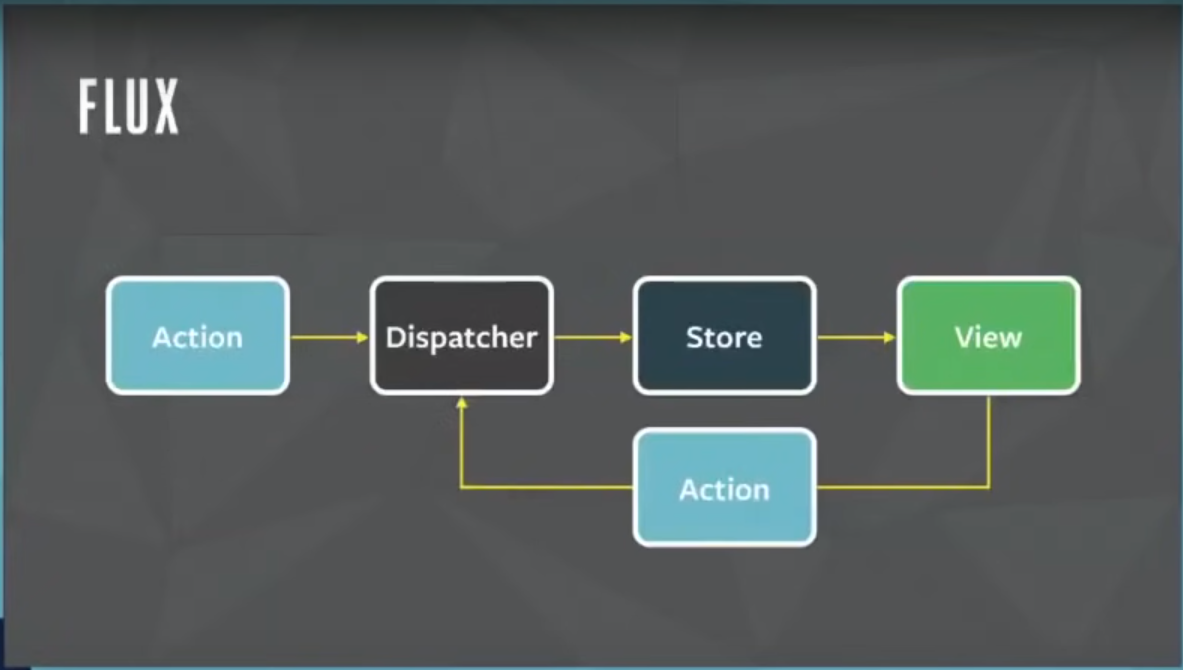
\includegraphics[width=10cm]{assets/flux.png} 

Fonte: Hacker Way: Rethinking Web App Development at Facebook(2014)

\end{figure}

% figura 1 end

% figura 1 start
\begin{figure}[htb]
\centering 
\caption{DIAGRAMA MVC EM PROJETOS DE GRANDE PORTE}
\setlength{\unitlength}{1mm}
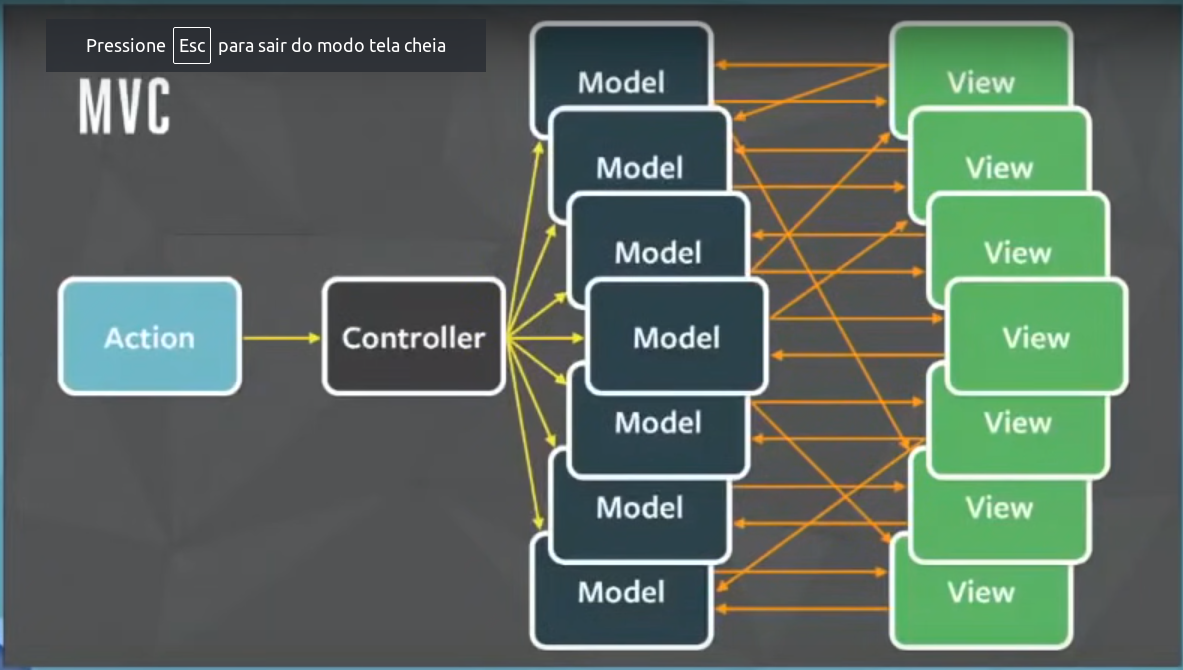
\includegraphics[width=10cm]{assets/mvc.png} 

Fonte: Hacker Way: Rethinking Web App Development at Facebook(2014)
\end{figure}
% figura 1 end

\subsection{Redux}
    O redux é uma biblioteca de gerenciador de estado amplamente utilizada, que implementa a arquitetura flux 

\subsection{React query}

O React query é uma biblioteca que facilita o consumo de Api's, o uso clássico para integrações com Api é utilizar um cliente http com as configurações de segurança e dados do sistema que se deseja integrar, obedecendo ao protocolo http para buscar os dados desejados, algumas fases da parte front-end se repetem ao tratar essa comunicação, existe uma ação do usuário como o click de um botão e então, se inicia a comunicação com o servidor(inicia-se um processo na aplicação de comunicação HTTP), espera-se a resposta mostrando para o usuário que algo assíncrono ocorre para que ele aguarde(renderização de um ícone ou texto que remeta carregamento), e após o recebimento dos dados do servidor, mostrar os dados ao usuário, tratando e fazendo algumas validações e formatações, o fluxo é ilustrado na Figura \ref{fig:fluxoRequisicao}. 

%figura 2 start
\begin{figure}[!h]
\centering 
\caption{FLUXO DE UMA REQUISIÇÃO A PARTIR DE AÇÃO DO USUÁRIO }
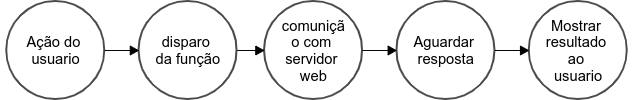
\includegraphics[width=16cm]{assets/Fluxo de requisição.png} 
{\footnotesize Fonte: Autoria própria (2023)}
\label{fig:fluxoRequisicao}
\end{figure}

%figura 2 end

O React query traz ferramentas genéricas prontas para facilitar o código desse processo, ele é um hook React, que implementa o tratamento desses estados de forma, no exemplo da figura \ref{fig:tratamentoDeEstados} possuímos um código extenso que em muitos projetos se repete em vários arquivos, já na figura \ref{fig:estadosComReactQuery} o exemplo do uso da biblioteca, é interessante focar na redução de complexidade para compreensão do código e na diminuição de linhas para o mesmo resultado.

\begin{figure}[!h]
\centering 
\caption{CÓDIGO PARA TRATAMENTO DOS ESTADOS}
\includegraphics[width=12cm]{assets/tratamentoDeEstados.png} 
{\footnotesize 

Fonte: https://blog.codeminer42.com/fetch-data-in-an-effective-way-with-react-query/}
\label{fig:tratamentoDeEstados}
\end{figure}

\begin{figure}[!h]
\centering 
\caption{UTILIZAÇÃO DO REACT QUERY PARA TRATAR ESTADOS E DADOS}
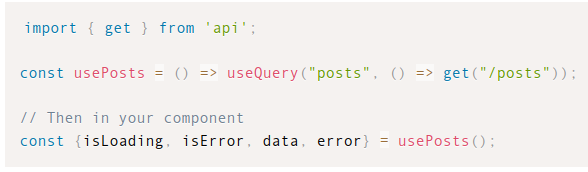
\includegraphics[width=15cm]{assets/estadosComReactQuery.png} 
{\footnotesize 

Fonte: https://blog.codeminer42.com/fetch-data-in-an-effective-way-with-react-query/}
\label{fig:estadosComReactQuery}
\end{figure}

A biblioteca recebe a requisição a ser feita, e a configuração da instância do dado, outra funcionalidade é o acesso global dos dados recebido no cache gerenciado na biblioteca, um dos problemas do React é compartilhar estados entre componentes, a biblioteca se mostra muito útil, pois facilita o tratamento de requisições de dados e os armazena, tendo isso em vista cada entidade dentro da aplicação é uma instância de hook react query, melhorando a organização. Outra vantagem é evitar requisições desnecessárias, que são um custo de infraestrutura. existe uma configuração em que é determinado o tempo que um dado fica obsoleto ou não, a partir dessa funcionalidade é possível implementar logicas em que um dado sempre esteja atual conforme a necessidade do usuário, porém com um custo menor.

\subsection{Typescript}
É uma ferramenta javascript que ajuda na identificação de erros na fase de desenvolvimento, pois,  adiciona tipagem a linguagem javascript, tornando a linguagem mais escalável e o código mais simples de ser entendido. O typescript é uma dependência javascript que não altera o funcionamento final de uma aplicação diretamente, é apenas uma ferramenta em tempo de desenvolvimento. Nas Figura \ref{fig:TypescritXJavascript}  que se encontra abaixo podemos ver um claro exemplo da diferença entre javascript puro e typescript, na figura da esquerda é instanciado a constante userJS que possui nome e senha, o javascript entende os tipos do objeto quando instanciado, porém, ao tentar acessar um campo inexistente, não existe aviso algum, o javascript entende que o campo pode ter sido adicionado ao objeto, na figura da direita um exemplo do que aconteceria no mesmo cenário utilizando typescript, ao acessar um campo inexistente a IDE com suporte, mostra um erro em tempo de desenvolvimento, com uma descrição clara do porquê existe um problema. 

%figura 2 start
\begin{figure}[h]
\centering
\caption{Exemplo em codigo diferença Typescript e Javascript}
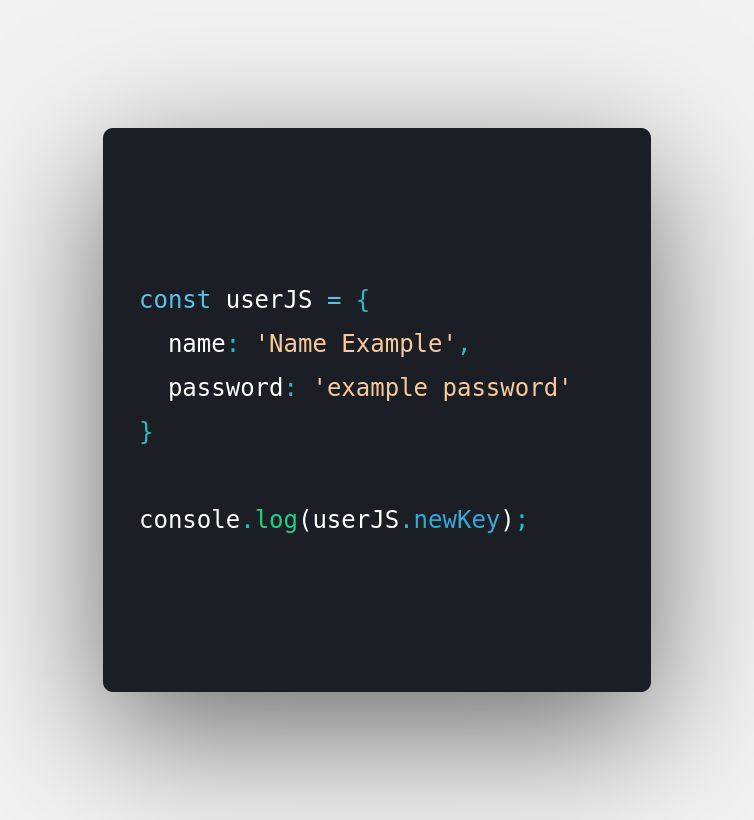
\includegraphics[width=8cm]{assets/codeJS.png} 
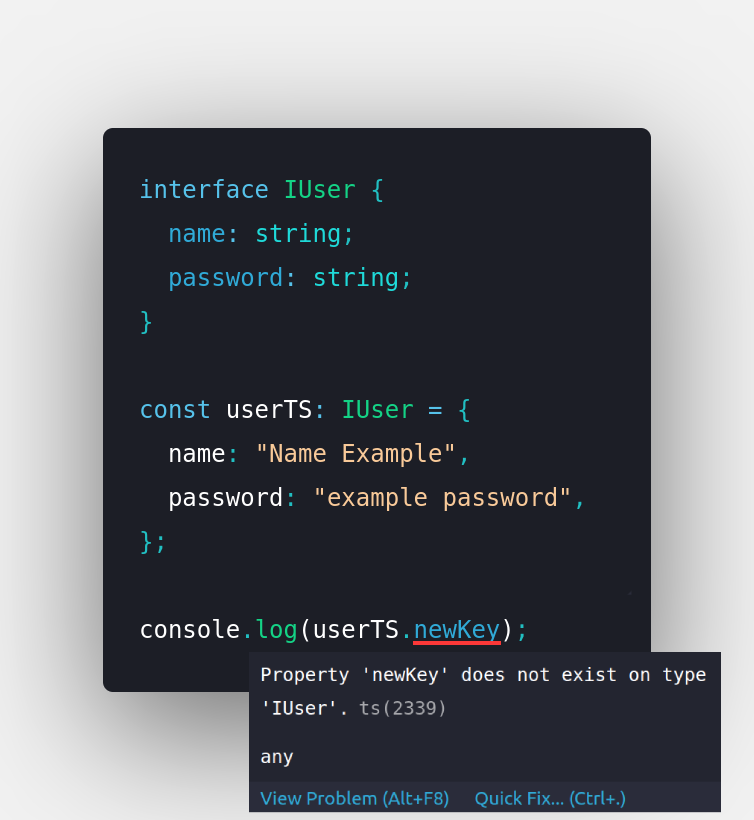
\includegraphics[width=8cm]{assets/codeTS.png}
{\footnotesize Fonte: Autoria própria (2023)}
\label{fig:TypescritXJavascript}
\end{figure}
Existem mais usos importantes da linguagem, que tornam um projeto muito mais escalável e fácil de ser compreendido, no caso de integrações com softwares via http, não se tem conhecimento se não documentado dos campos de um objeto, o typescript, ajuda a documentar quais atributos do objeto recebido podem ser acessados, e evita erros de escrita que não seriam percebidos até um erro na aplicação já em runtime, perceber os erros em desenvolvimento, acelera e torna mais dinâmica a criação de funcionalidades em um aplicativo, agregando assim valor ao software final.

\subsection{Styled components}

Styled components é uma biblioteca javascript que auxilia na criação de estilos CSS para os elementos visuais, ele permite a criação de componentes estilizados o que se encaixa muito bem na estrutura e logica do react, também é possível adicionar logica a esses componentes melhorando o encapsulamento do projeto mantendo validações de estilização dentro do componente, um componente de estilo da biblioteca pode ser reutilizado em vários lugares a depender da qualidade e de o quão genérico ele é, o que melhora a reutilização de código e aumenta a velocidade de desenvolvimento das aplicações. No React native ele substitui o StyleSheet, que é semelhante aos modelos mais clássicos de estilização CSS da Web, nele se torna mais verboso a criação de estilos condicionais, e sua sintaxe requer mais código no geral.

\subsection{Native base}

É uma biblioteca de componentes visuais genéricos e de fácil edição react native que auxilia no desenvolvimento de interfaces, a biblioteca utiliza o conceito de programação declarativa "tem seu foco em descrever o resultado desejado e como ele deve se parecer, ao invés de listar todos os passos de execução até se obter este resultado."(Nicholas Segger,2021), no conceito UI declarativa os estilos de um componente do react native tradicional, os estilos são definidos caso a caso, e não são vinculados a um componente específico, geralmente existe um arquivo só para a declaração desses estilos, em grandes aplicações, desenvolvidas por equipes, é comum a criação de um código que já existe, o que torna a aplicação mais carregada. na UI declarativa as estilizações descritos na sua instância, que diminui código e evita redundância acidental de código.  

\subsection{MVVM}
 É um padrão de design um pouco mais semelhante aos tradicionais do que o flux, o princípio do padrão é separar a lógica do que e interface do usuário

\section{ Bee comerciais - Desenvolvimento de aplicativo para uso interno}
O setor comercial na empresa Bee delivery é o responsável pelo relacionamento entre os clientes da bee delivery e a empresa, nessas atividades existe a demanda de gerenciar os dados de captação de clientes, agendamento de visitas entre outros, o aplicativo dos comerciais foi pensado para complementar o sistema já existente que possuía algumas funcionalidades das citadas anteriormente, já que foi relatado uma certa dificuldade de usabilidade da aplicação web, tendo em vista que os usuários na maioria do tempo utilizavam por dispositivos moveis. 

\subsection{Projeto}
Tendo em vista essas necessidades iniciou-se o processo de engenharia de software da aplicação, onde participei como observador das primeiras etapas, e ativamente na etapa de desenvolvimento da parte front-end mobile do projeto, nesta seção será descrito o processo de software observado, da demanda até o usuário final. A bee como uma startup tem um modelo acelerado de negócio, devido a isso o produto inteiro levou cerca de 4 meses para ser completo, o projeto era um MVP(mínimo produto viável) o que tornou esse tempo de execução possível, e é um modelo muito utilizado quando se precisa ter resultados e validar as necessidades do usuário no menor prazo possível.

\subsection{Participantes e papeis}

Como atores do processo podemos descrever: o cliente, que tinha o papel de exigir prazos, e requisitos de software, acompanhar o processo de desenvolvimento por meio de apresentações de produto, e realizar as sugestões de mudança caso necessário, tudo isso com um baixo nível de influência na parte de realização, o ux/ui responsável em desenvolver as telas dos fluxos determinados, o Product Manager responsável na metodologia Scrum por ser a primeira camada entre cliente e a equipe de desenvolvimento, as descrições e divisões das demandas para os setores responsáveis.

\subsection{Validação de requisitos}

O modelo de elicitação e validação de requisitos foi feita por um funcionário do setor de UX/UI com a metodologia de prototipação juntamente com a funcionária Product Owner que decide em último caso qual a melhor solução para determinado problema, na prototipação é feito uma aplicação com funcionalidades semelhantes a um software, porém muito limitado, o ponto positivo da prototipação é que o tempo de desenvolvimento é menor e pode-se visualizar do fluxo e encontrar falhas ou melhorias, além disso, o processo de prototipagem em empresas com um UX/UI é sempre realizado, o que economiza passos em comparação a outros meios de validação de requisitos.O protótipo após terminado era constantemente exposto a pesquisas internas a fim de ver na prática o funcionamento, e a usabilidade dos fluxos determinados, nessa fase o produto pode passar por várias alterações a fim de atender as necessidades e as sugestões da pesquisa podem solucionar alguns problemas de usabilidade com mais facilidade. 

\subsection{Primeira etapa do desenvolvimento}

O projeto seria um aplicativo integrado com o sistema de usuários da bee delivery já existentes, e o 
desenvolvimento da parte do sistema de back-end não estava inicialmente pronta, com os requisitos definidos, e o protótipo completo e validado pelo cliente e Product Owner, foi iniciado o desenvolvimento das telas em react native, inicialmente não foi pensada uma arquitetura de organização de pastas, porém tendo em vista a maioria dos padrões de projeto deixa a camada de interfaces de usuário desacoplada da lógica, a primeira etapa se encaixou corretamente sem gerar nenhum retrabalho futuro, foram desenvolvidas as telas do fluxo, utilizando mocks, que são dados simulados estáticos, para simular a manipulação de dados real da aplicação final, já visando as etapas posteriores.

\subsection{Segunda etapa do desenvolvimento}
o segundo passo foi a interação com o desenvolvedor responsável pela criação dos endpoints que seriam integrados pelo aplicativo, o método de comunicação foi validação dos dados necessários, e quais recursos seriam interessantes, por exemplo, no aplicativo são listadas visitas agendadas que um usuário ira fazer, por data, então a solução foi uma paginação por data uma consulta informa um dia, e as credenciais de segurança para a api, e recebe como resposta somente a lista de visita de um dia em específico, em geral, a paginação é uma estratégia padrão de uma api rest, mas nesse exemplo prático, em um cenário de uma quantidade grande de visitas, esse tipo de consulta economiza recursos no banco de dados tendo em vista que tem mais critérios, possibilitando uma otimização da query no banco, buscando somente em certo intervalo de linhas, e não resultando em nenhuma perda de funcionalidade ao cliente, atendendo ao requisito de sistema que é: listar visitar por intervalo de tempo de um dia.


\subsection{Conclusão do desenvolvimento}
Com a documentação dos endpoints em mão foi iniciado o trabalho de integração do front-end com os dados reais do sistema, os mocks tornaram o processo mais rápido tendo em vista que os dados no código estavam centralizados em uma variável, a biblioteca utilizada para integração foi o React Query, uma biblioteca de gerenciamento de estado assíncrono, o uso dessa ferramenta na empresa era inicial, onde os desenvolvedores realizam estudos da biblioteca, utilizam em projetos paralelos ao código para averiguar se atende a demanda de produtividade, desempenho e qualidade necessária para o projeto dos aplicativos, na aplicação trabalhada, existiam 3 camadas a de lógica interna do aplicativo, os dados externos e as definições visuais, como o escopo era reduzido, somente 2 camadas foram necessárias, uma visual a View, que carregava também a pouca lógica necessária para validações visuais,e a camada de dados a Model, que era a camada com a integração de dados da api e a manipulação dos mesmos para serem renderizados em tela.

%figura 3 start
\begin{figure}[h]
\centering 
\caption{ARQUITETURA UTILIZADA NA APLICAÇÃO DOS COMERCIAIS}
\hspace*{-1.5in}

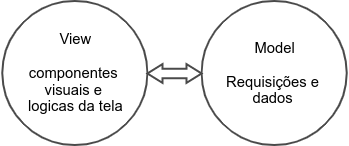
\includegraphics[width=10cm]{assets/arquiteturaSimples.png} 

Fonte: Autoria própria (2023)
\end{figure}

%figura 3 end

Fonte: Autoria própria (2023)


Um dos requisitos de sistema era realizar a checagem da posição do usuário, ao da baixa em uma visita era validada a posição do usuário em relação à empresa visitada, essa lógica foi feita utilizando recursos do react native, que oferece integrações a recursos dos sistemas operacionais Android e IOS obedecendo aos protocolos de cada plataforma, é necessário pedir permissão do usuário para poder consultar a localização do mesmo do seu dispositivo, após essa configuração a biblioteca  Geolocation na época do próprio react native, hoje ‘react-native-community/geolocation’ mantida pela comunidade, facilita a implementação onde um código só consulta a localização do dispositivo para android e ios. Com esse processo e organização foi possível realizar a entrega do projeto em 3 meses, contando validação dos fluxos e projeto, e desenvolvimento do front-end e back-end e já está nas lojas App store e Play store sendo utilizado, o projeto era trabalhado em paralelo a projetos maiores já vigentes na empresa, o que mostra que o processo de produção obteve sucesso em termos de desempenho e velocidade.

\subsection{Fluxo de integração e distribuição}

Ao terminar o desenvolvimento foi implementado um fluxo de distribuição para a aplicação, é normal para as empresas implementarem esse fluxo, apesar de ser possível criar um pacote localmente na própria maquina usada para o desenvolvimento, o processo é passível de falhas, um fluxo de distribuição e integração implementa um protocolo que dificulta erros, a ferramenta utilizada foi o appcenter da microsoft já instalado na aplicação, o fluxo manual após a equipe concluir uma certa quantidade de demandas, por meio de um gerenciador de versão de código é realizada uma mescla dessas demandas em uma ramificação que contem as funcionalidades necessárias para uma nova versão da aplicação, com versão e configuração de arquivos atualizada, com essa versão é compilado para um pacote compatível com a app store ou apple store, e feito o upload manualmente nos serviços das mesmas. No fluxo automatizado, ao concluir e mesclar as versões utilizando um gerenciador de versão de código, o app center escuta essa alteração e configura as atualizações necessárias de versão, cria um pacote para as lojas e os pública, existe uma otimização no tempo dos desenvolvedores e um ganho de tempo e qualidade das aplicações.  a figura X abaixo ilustra o processo de desenvolvimento contínuo.
\section{Bee para entregadores - Melhorias no código do aplicativo motoboy.}

O aplicativo dos motoboys da bee delivery Bee delivery para Entregadores, disponível na Playstore com mais de 1 milhão de downloads é o objeto de trabalho a ser explorado neste tópico, utiliza a tecnologia React native e é por onde os motoboys recebem as demandas de entregas, esses chamados acontecem em tempo real utilizando o serviço Firebase Cloud Messaging utilizado para todas as atualizações onde o cliente(usuário entregador) seja um ator passivo, um dos fluxos que pode exemplificar é uma empresa chama motoboys e estes recebem em seu celular uma mensagem do sistema com as informações da entrega, o motoboy pode aceitar ou recusar a entrega informando para o sistema por meio de requisições http comuns, 
\subsection{Ambiente tecnológico inicial}
\subsection{Melhorias no ciclo de distribuição da aplicação.}
\subsection{Redução de requisições}
\subsection{Conhecimentos adquiridos com outras equipes}
\subsection{Resultados finais}

Todas as tecnologias citadas acima são utilizadas hoje no projeto em que vivencio, existe um processo de migração da estrutura antiga com flux e redux, para uma nova estrutura que utiliza react query, native base e mvvm.


\section{Reflexão por parte do aluno sobre as principais contribuições ao projeto}
ESCREVER.

implatação de um padrão auxiliar
discusão sobre novos objetivos no software
foco em redução de custos e manutenção do codigo

\section{Relação dos principais conhecimentos obtidos nas disciplinas do curso e que foram de importância para o estágio}
As disciplinas do curso de Ciências da Computação tiveram grande importância para a base do conhecimento utilizado no ambiente real da empresa, apesar de não utilizar nenhuma das vistas nas das tecnologias disciplinas aprofundadamente, os conceitos mais tradicionais de programação são utilizáveis nas tecnologias e paradigmas atuais,  os conceitos mais avançados vistos na disciplina de Poo que tratam de encapsulamento de dados e escalabilidade, foram importantes para ter a noção de reaproveitamento de código utilizando padrões de projeto e aplicando as boas práticas,  criar softwares escaláveis e bem organizados arquiteturalmente, na disciplina foi realizado um projeto com o padrão MVC, criando  uma familiaridade com esses padrões de projeto, e por ser mais tradicional e ser base de outros padrões facilita muito aprende antes de partir para os padrões específicos como o Flux, o paradigma do React é diferente do java por utilizar o paradigma funcional, porém o padrão MVVM utilizado para lógicas mais simples nos projetos da empresa, é semelhante ao MVC, o padrão utilizado pela equipe do Facebook antes da criação do flux era o MVC então existe uma contribuição da base geralmente. 

Outra grande contribuição foi a disciplina de programação básica, tendo foco em desempenho do software, onde é possível manipular espaços de memória e ter noções sobre como evitar vazamentos de memória, o primeiro contato com a criação de algoritmos mais eficientes em termos de desempenho, e ter noções de linguagens mais próximas ao hardware, no desenvolvimento React native, por utilizar o paradgima funcional, tende se a pensar na produtividade acima do desempenho, os exemplos da comunidade geralmente implementam laços de repetições desnecessários, e outras más práticas que pode ser melhor observado na disciplina.

As disciplinas de sistemas operacionais e arquitetura de computadores fornece as noções sobre limitações de hardware e quais estrategias são utilizadas para organizar as tarefas dos softwares de forma eficiente em um SO, e mostra também alguns algoritmos clássicos que podem ser utilizados em várias situações, o que faz importante ter conhecimento sobre, uma aplicação mobile lida diretamente com o sistema operacional o Android e IOS, em desenvolvimento é normal configurar e utilizar frequentemente uma máquina virtual que simula um smartphone, um exemplo de sistema operacional virtual, estudado nas aulas ministradas no curso.  

Engenharia de software, gestão de projetos e elicitação de requisitos contribui para o profissional no mercado de trabalho, em termos de organização de software, nota-se uma grande negligência com a parte de documentação, e toda parte inicial do processo de engenharia, um bom profissional entende o porquê dessa negligência e tenta adaptar novos processos, entender o que já funciona e o que pode melhorar, além de entender as metodologias ágeis, O State of Scrum 2017-2018 ao fazer o levantamento apontou que 83\% das empresas utilizam scrum de forma hibrida com alguma outra metodologia, dominar essas metodologias é indispensavel para o profissional da área.

\section{Reflexão sobre as dificuldades enfrentadas pelo estagiário na organização}
  Inicialmente o maior impacto foi a falta de referência para a programação em react native,  o aluno de computação aprende várias linguagens diferentes, porém poucas disciplinas, utilizam o javascript ou outra linguagem mais voltada a web, em sua maioria as linguagens mais utilizadas foram c++ e java, os conhecimentos adquiridos para passar no teste técnico da empresa foram adquiridos estudando por conta própria, com a criação de aplicativos e cursos online,  com os conhecimentos de programação básica e POO a dificuldade estava na diferença de paradigma e como a comunidade React utiliza o javascript mais moderno, foi difícil adaptar os conceitos de escalabilidade aprendidos em POO, nos projetos, e também difícil entender a arquitetura flux. 

Um código de uma aplicação que é um produto de startup, em que uma equipe desenvolve, foi um tanto desafiador no sentido de entender os padrões internos utilizados, os artigos da comunidade muitas vezes são superficiais, no nível avançado, raramente se encontra um material de qualidade sobre aplicações escaláveis, ao contrário do java com muita coisa definida que funciona, o react ainda está amadurecendo, e muita coisa ainda está sendo desenvolvida, isso é um grande desafio também para os desenvolvedores.

Existiu também uma dificuldade de saber onde a teoria se aplicava na prática, as disciplinas isoladas não deixavam claras onde cada conhecimento é utilizado por uma empresa, o que um software utiliza em cada nicho, os conceitos de uma arquitetura monólito, banco de dados e outros, não tinham destino antes de uma grande preparação para o mercado de trabalho, o estudante de computação é um profissional muito versátil para o mercado de trabalho por ter conhecimento em quase todas as áreas do software, porém faltam mais exemplos reais, para direcionar os esforços de estudos para o aplicável na sociedade.   

\section{Relação de tópicos que poderiam ser estudados no curso de Computação e que foram necessários no estágio.}
ESCREVER.

tópicos sobre protocolo http

criação de software seguro

programação web aprofundada com o uso de frameworks

empreendedorismo voltado a computação


\end{document}

